\section{VHDL}
\subsection{Introducción}
VHDL es un lenguaje de descripción de circuitos electrónico digitales que utiliza distintos niveles de abstracción. Creado en 1980 por 
el DoD\footnote{\textit{Department of Defense}} de Estados Unidos y el IEEE. Acrónimo de ``VHSIC\footnote{\textit{Very High Speed 
Integrated Circuit}} Hardware Description Language''.

El lenguaje tiene las siguientes características:
\begin{itemize}
 \item Los diseños pueden descomponerse jerárquicamente.
 \item Cáda elemento del diseño tiene una interfaz bien definida (para conectarla a otros elementos) como una especificación de 
comportamiento precisa (para simularla)
 \item El comportamiento puede ser especificado por un algoritmo o bien por una estructura de hardware real.
 \item La concurrencia, temporización y señales de reloj pueden ser todas modeladas.
 \item La operación lógica y comportamiento de temporización de un diseño pueden simularse.
\end{itemize}

VHDL comenzó como un lenguaje de modelado y documentación. Si bien esto fue una innovación importante, el salto cuántico lo obtuvo con 
el desarrollo de herramientas de síntesis VHDL. Estos programas tienen la capacidad de crear circuitos lógicos a partir de su descripción
en hardware. Con VHDL se puede simular y sintetizar cualquier circuito combinacional simple hasta un ``microprocesador completo''.

VHDL en si no es un lenguaje de programación, por lo tanto no alcanza con conocer su sintaxis. Para diseñar en VHDL hay que:
\begin{itemize}
 \item Pensar en puertas y biestables, no en variables o funciones.
 \item Evitar bucles combinacionales y relojes condicionados.
 \item Saber qué parte del circuito es combinacional y cuál secuencial.
\end{itemize}

El objetivo final de escribir código en VHDL es poder diseñar circuitos que se puedan implementar en circuitos integrados de lógica
programable como CPLD o FPGA's.

\subsection{Estructura de programa}
Los archivos generados en VHDL (extensión .vhd) tienen la descripción del circuito que se quiere implementar. Viéndolo a nivel macro, 
nos encontraremos con dos grandes bloques como se observa en la Figura \ref{vhdlbloque}

\begin{figure}[h]
  \centering
    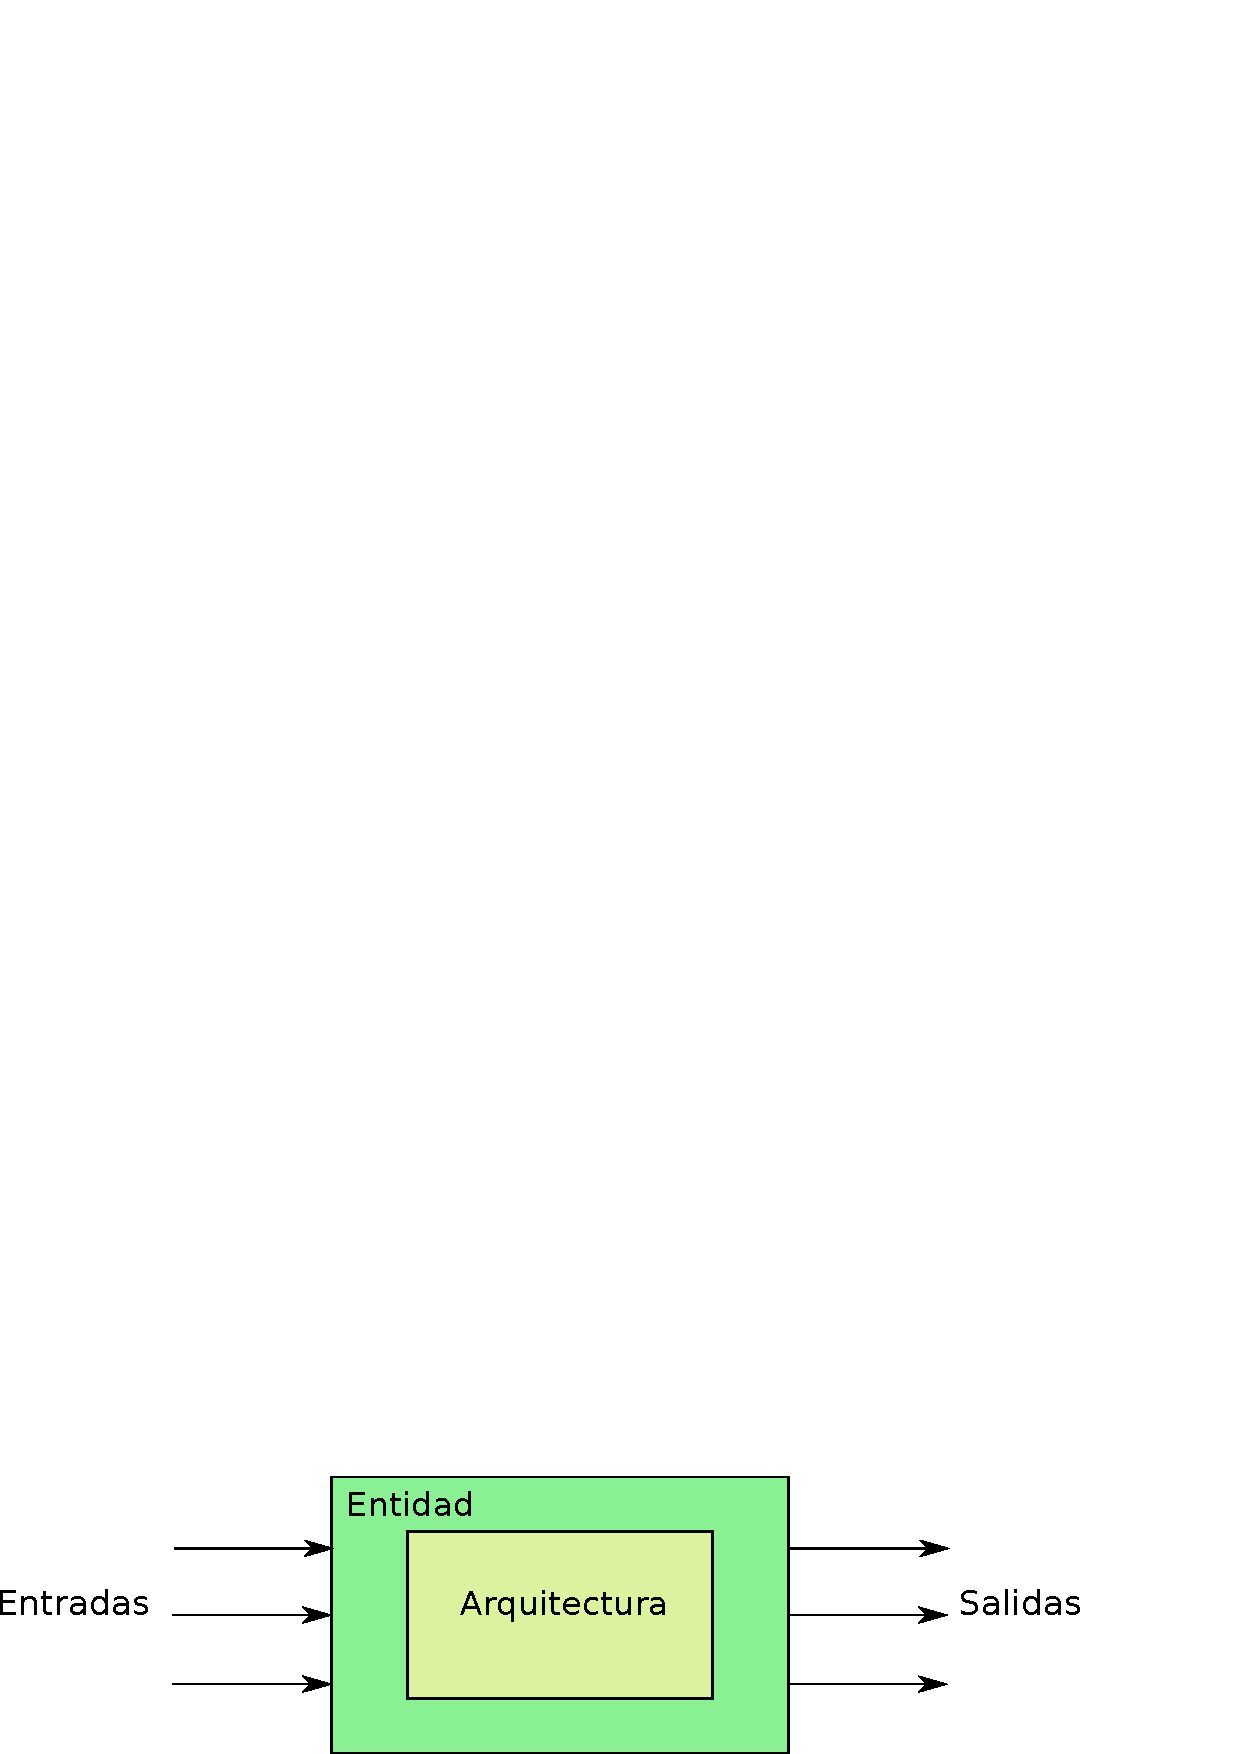
\includegraphics[width=.85\textwidth]{graficos/vhdl.pdf}
  \caption{Estructura VHDL}
  \label{vhdlbloque}
\end{figure}

\subsubsection{Entidades (Entity)}
La entidad describe únicamente la forma externa del circuito. Es el lugar donde se enumeran las entradas y salidas del diseño.
Podríamos imaginarnos a una entidad como un símbolo esquemático de un diagrama electrónico, el cual describe las conexiones del 
dispositivo hacia el resto del diseño.
La Figura \ref{entidad} describe gráficamente este concepto.

\begin{figure}[h]
  \centering
    \includegraphics[width=.5\textwidth]{graficos/entidad.pdf}
  \caption{Entidad VHDL}
  \label{entidad}
\end{figure}


\begin{lstlisting}[style=vhdl]
entity Mi_Entidad is
     port (Entrada_A,Entrada_B : in  bit;
           Salida_A,Salida_B   : out bit)
end Mi_Entidad
\end{lstlisting}

\subsubsection{Arquitectura (Architecture)}
La arquitectura es una detallada descripción del comportamiento o estructura interna del módulo. Si vemos a la entidad como una caja 
negra en la que se enumeran las interfaces de conexión, la arquitectura representa la estructura interna de dicha caja.

\begin{lstlisting}[style=vhdl]
architecture Nombre_arquitectura of Mi_entidad is
--declaracion de senales;
begin
--Sentencias concurrentes (combinacionales)
--Sentencias secuenciales
   process (lista de sensibilidad)
   --declaracion de variables;
   begin
     --sentencias
   end process;
end nombre_arquitectura
\end{lstlisting}

\subsubsection{Identificadores}

\paragraph{Constant}
Los objetos de esta clase tienen un valor inicial que es asignado de
forma previa a la simulación y que no puede ser modificado durante ésta.
\begin{lstlisting}[style=vhdl]
 constant identificador: tipo:= valor;
\end{lstlisting}

\paragraph{Variable}
Los objetos de esta clase contienen un único valor que puede ser
cambiado durante la simulación con una sentencia de asignación. Las variables
generalmente se utilizan como índices, principalmente en instrucciones de bucle, o
para tomar valores que permitan modelar componentes. Las variables NO
representan conexiones o estados de memoria.
\begin{lstlisting}[style=vhdl]
 variable identificador: tipo [:= valor];
\end{lstlisting}

\paragraph{Signals}
Los objetos de esta clase contienen una lista de valores que incluye el
valor actual y un conjunto de valores futuros. Se las puede ver como los
``cables'' de interconexión de elementos. Las señales representan elementos de
memoria o conexiones y sí pueden ser sintetizadas. Los puertos de una entidad son
implícitamente declarados como señales en el momento de la declaración, ya que
estos representan conexiones. También pueden ser declaradas en la arquitectura
antes del BEGIN, lo cual nos permite realizar conexiones entre diferentes módulos.
\begin{lstlisting}[style=vhdl]
 signal identificador: tipo;
\end{lstlisting}

\subsubsection{Tipos y constantes}

Todas las señales, variables y constantes en un programa VHDL deben tener un ``tipo''
asociado. El tipo especifica el conjunto o intervalo de valores que el objeto puede tomar.
y también hay típicamente un conjunto de operadores (suma, ANO, etc.) asociados con un tipo dado.

A continuación se describirán algunos de los tipos mas utilizados:

\paragraph{BIT}
Puede tomar los valores ``0'' y ``1''.

\paragraph{BIT\_VECTOR}
Agrupación de bits. Por ejemplo:

\begin{lstlisting}[style=vhdl]
signal salida : BIT_VECTOR (0 to 3);
salida <="1000";
\end{lstlisting}

esto significa que:

salida(0)=``1''

salida(1)=``0''

salida(2)=``0''

salida(3)=``0''

\paragraph{INTEGER}
A veces utilizado para índicesde loops, constantes, valores genéricos, etc.

\paragraph{BOOLEAN}
Puede tomar los valores ``true'' o ``false''

\paragraph{STD\_LOGIC}
Los dos valores del tipo ``Bit'' no alcanzan para definir todos los estados que puede tomar una señal digital.
No es un tipo propio de VHDL, es un tipo definido en la librería IEEE.standard\_logic\_1164.

La tabla \ref{std_logic} describe los posibles valores que pueden tomar.

\begin{table}[!hbt] 
\centering
 \begin{tabular}{|c|c|}
\hline
U & No inicializado, valor por defecto. \\ \hline
X & Desconocido fuerte, salida con múltiples fuentes en corto \\ \hline
0 & Salida de una puerta con nivel lógico bajo \\ \hline
1 & Salida de una puerta con nivel lógico alto \\ \hline
Z & Alta Impedancia \\ \hline
W & Desconocido débil, terminación de bus \\ \hline
L & 0 débil, resistencia de pull-down \\ \hline
H & 1 débil, resistencia de pull-up \\ \hline
\end{tabular}
  \caption{Valores de Std\_Logic}
  \label{std_logic}
  
\end{table}      

\paragraph{STD\_LOGIC\_VECTOR}
Se utiliza para describir buses, es un array de ``Std\_Logic''.

\subsubsection{Operadores}
Los operadores integrados para los tipos ``integer'' y ``boolean'' se enumeran en la tabla \ref{operadores}.

\begin{table}[!hbt] 
\centering
 \begin{tabular}{|c|c|c|c|}
\hline
\multicolumn{2}{|c|}{\textbf{Operadores Integer}} & \multicolumn{2}{|c|}{\textbf{Operadores Boolean}}\\ \hline
+   & Suma               & and   & AND  \\ \hline
-   & Resta              & or    & OR   \\ \hline
*   & Multiplicación     & nand  & NAND \\ \hline
/   & División           & nor   & NOR  \\ \hline
mod & División entera    & xor   & XOR  \\ \hline
rem & Residuo            & xnor  & XNOR \\ \hline
abs & Valor absoluto     & not   & NOT  \\ \hline
**  & Exponencial        &       &      \\ \hline


\end{tabular}
  \caption{operadores}
  \label{operadores}
  
\end{table}    

\subsection{Descripción de comportamiento}
\subsubsection{PROCESS}
Un PROCESS es una sentencia concurrente, esto significa que si tenemos varios PROCESS (y se dan las condiciones adecuadas), los mismos 
se ejecutarán al mismo tiempo. No obstante las sentencias que hay dentro del PROCESS se ejecutan de forma secuencial. Es la única forma
que tenemos en VHDL de ejecutar algo en forma secuencial.

Por lo tanto se puede decir que una estructura secuencial va en el interior de un PROCESS.

La estructura genérica de esta sentencia es:

\begin{lstlisting}[style=vhdl]
 PROCESS [lista de sensibilidad]
       --declaracion de variables
     BEGIN
       --sentencias secuenciales
     END PROCESS;
\end{lstlisting}

La lista de sensibilidad \footnote{La lista de sensibilidad solo funciona en simulación, cuando se implemente el hardware, 
se deben utilizar otras técnicas} es una serie de señales que, al cambiar de valor, hacen que se ejecute el PROCESS.

Un ejemplo sería:

\begin{lstlisting}[style=vhdl]
 PROCESS(signal1, signal2)
     ...
\end{lstlisting}

\subsubsection{WAIT}
Se utiliza para reemplazar la lista de sensibilidad

\begin{lstlisting}[style=vhdl]
 wait on signal_list;
 wait for time_expression;
 wait until condition;
\end{lstlisting}

Los eventos sobre las señales (‘EVENT) nos indican cuando ocurre un cambio en la señal
\begin{lstlisting}[style=vhdl]
signal'event
signal'last_event
signal'last_value
\end{lstlisting}


\subsubsection{IF – THEN – ELSE}
Sólo son aplicables dentro de un process
\begin{lstlisting}[style=vhdl]
if condicion then
   ...
   --sentencias secuenciales
elsif otra_condicion then
   ...
   --sentencias secuenciales
else
   ...
   --sentencias secuenciales
end if;
\end{lstlisting}

\subsubsection{CASE – WHEN} 
Sólo son aplicables dentro de un process
\begin{lstlisting}[style=vhdl]
case expresion is
   when alternativa_l =>  ... --sentencias sec.
   ...
   when alternativa_n =>  ... --sentencias sec.
   when others =>         ... --sentencias sec.
end case;
\end{lstlisting}

\subsubsection{FOR – LOOP}
Sólo son aplicables dentro de un process
\begin{lstlisting}[style=vhdl]
for loop_var in range loop
    ... --sentencias secuenciales
end loop; 
\end{lstlisting}

\subsubsection{WHILE – LOOP}
Sólo son aplicables dentro de un process
\begin{lstlisting}[style=vhdl]
 while condicion loop
    ... --sentencias secuenciales
end loop;
\end{lstlisting}

\subsubsection{WHEN – ELSE}
Sólo son aplicables dentro de un process
\begin{lstlisting}[style=vhdl]
 Signal_name <= valor_1 when condicion1 else
                valor_2 when condicionn2 else
                ...
                valor_i when condicioni else
                otro_valor;
\end{lstlisting}

\subsubsection{WITH – SELECT – WHEN}
Sólo son aplicables dentro de un process
\begin{lstlisting}[style=vhdl]
 with identificador select
 Signal_name <= valor_1    when valor_identificador1,
                valor_2    when valor_identificador2,
                ...
                valor_i    when valor_identificadori,
                otro_valor when others;

\end{lstlisting}
